%!TEX TS-program = pdflatex
%!TEX encoding = UTF-8 Unicode
%!TEX options = --shell-escape -synctex=1 -interaction=nonstopmode -file-line-error "%DOC%"
\documentclass[final]{kuee_en}

\usepackage[final,breaklinks=true]{hyperref}
\renewcommand*{\sectionautorefname}{Section}

\usepackage[nomarkers,
    % disable,
    ]{endfloat}
\renewcommand{\efloatseparator}{\mbox{}}

% \usepackage{cleveref}

% \usepackage[final]{hyperref}

\usepackage{xcolor,graphicx}
\usepackage{subcaption}
\usepackage{sectsty} % change section style
\sectionfont{\noindent\textsc} % indent setting
% \usepackage{paralist}
% \usepackage{booktabs}
\usepackage[utf8]{inputenc}
\usepackage[T1]{fontenc}
\usepackage{tgbonum}
\usepackage{fancyhdr}
% \usepackage{tocloft}

\usepackage[inkscape=on]{svg}
\svgpath{{imgs/svg/}}
\usepackage[off]{svg-extract}
\svgsetup{%
	extractpath=./imgs/svg-extract/,
	inkscapepath=./imgs/svg-inkscape, 
	clean=true,
	convertformat={png},
	convertdpi={png=600},%
	convertdpi=300}

% \renewcommand{\cftsetpnumwidth}{3em}% Default is 1.55em
% \renewcommand{\cftchapfont}{\bfseries\raggedright}% Default is \bfseries

%%%%%%%%%% Start TeXmacs macros
\newcommand{\mathd}{\mathrm{d}}
\newcommand{\tmname}[1]{\textsc{#1}}
\newcommand{\tmop}[1]{\ensuremath{\operatorname{#1}}}
\newcommand{\tmtextit}[1]{{\itshape{#1}}}
\newcommand{\nosymbol}{}
\newcommand{\tmmathmd}[1]{\ensuremath{#1}}
%%%%%%%%%% End TeXmacs macros


\etitle{Broadband frequency entangled photon generation using silicon nitride ring cavities}
% \title{\cjk{窒化シリコンリング共振器を用いた\\広帯域周波数もつれ光子生成}}
\title{Broadband frequency entangled photon generation using silicon nitride ring cavities}
\eauthor{Zhenghao Yin} 
\author{\cjk{殷 政浩}}
\supervisor{\cjk{竹内 繁樹 教授}}
\school{\cjk{京都大学大学院工学研究科}}
\depart{\cjk{電子工学専攻}}
\date{\cjk{令和2年2月1日}}

\begin{document}
\maketitle

\begin{abstract}
    \lipsum[1]
\end{abstract}

\tableofcontents
% \clearpage


% !TeX root = ../main.tex
\chapter{Introduction}

\section{Background}

Quantum mechanics has not only boosted up the modern science and technology in different disciplines, but also established the cornerstone for future quantum information processing technology. 
Furthermore, differing from the past applications of quantum mechanics which only involves the quantization nature, the frontier quantum information processing 
including but not limited to quantum computation, quantum communication and quantum metrology, 
exploits the deep-level physics of quantum mechanics, such as quantum superposition and quantum entanglement.
Therefore, the fundamental quanta of light---photon---featuring attractive advantages like long coherent time and multiple degrees of freedom (DoF), is a suitable candidate among the research quantum computation and quantum communication. 

Furthermore, entanglement between photon pairs which originates from the nonlocality of quantum mechanics, can be easily realized using nonlinear bulk crystals. 
While in the term of DoF, much of research up to now focuses on the polarization and path entanglement approaches and very little attention has been paid to frequency entanglement, whose basis is continuous and infinite in hilbert space. 
Moreover, the previous research shows that frequency entangled photon pairs can be exploited not only in wavelength division multiplexing quantum key distribution \cite{Wengerowsky2018} but also promising to transfer quantum information in future quantum networks \cite{Tchebotareva2019}. 
An example of quantum computation is cluster state encoded by frequency \cites{Reimer2019}.
Therefore, frequency entangled photon plays a powerful and general role for optical quantum information processing.

Nevertheless, large scale realization of frequency entanglement requires hundreds of free-space optical components, especially the nonlinear crystals, which challenges robust manipulation of generated quantum states.
Besides, in recent applications of quantum metrology, quantum optical coherent tomography (QOCT), the broadband frequency entanglement \cite{Okano2015} is also urgent.

To improve both scalability and robustness, chip-scale full-optical routine has been developed for optical quantum information processing \cites{ Vahala2008, OBrien2009}.  
A conventional material candidate is silicon on insulator (SOI), since it is CMOS compatible and supplied by silicon wafer manufacturers. Much of research up to date reported not only frequency \cite{Kues2017b} but also path and time-bin encoded quantum state in this platform \cites{Paesani2018,Zhang2018a}. Other materials like lithium niobate and aluminum nitride are also developed and show various advantages, but requires special fabrication technology.

\section{Objective}

However, suffering from two photon absorption and stimulated Raman scattering \cite{Engin2012}, silicon is no able to generate high-intensity and broadband frequency conversion. 
Since that, silicon nitride, which is transparent from visible to near infrared range, can be used to achieve ultra-broadband frequency conversion. 
A simple comparison of these two material is shown in \autoref{tab:si-vs-sin}.
Recently, single photon pair generation from visible to telecom band is reported\cite{Lu2016}. 

\begin{table}[]
	\mycaption{Comparison of several material properties between silicon and silicon nitride}{The data of silicon is cited from Reference \cite{Sinclair2019} and silicon nitride refers to \cite{Ang2018}.}
	\label{tab:si-vs-sin}
	\begin{tabular}{ccc}
							& silicon nitride 			& silicon		 			\\ \hline
		refractive index $n$ at 1550 nm
							& 2.0						& 3.4						\\ \hline
		transparent band 	& visible to NIR			& NIR					    \\ \hline
		two photon absorption $ \beta_\mathrm{TPA} $ (cm/GW)                 
							& - 						& 0.75 			 			\\ \hline
		Kerr nonlinearity $ n_2 $ (\si{\square\meter\per\watt})             
							& \num{6.94d-19} 			& \num{5d-18} 				\\ \hline
	\end{tabular}
\end{table}

In the silicon nitride waveguide, third-order optical nonlinearity is dominant and leads spontaneous four wave mixing in sub-micron scale. 
To enhance the nonlinear interaction, the all-pass ring resonator is used where the light is coupled inside from a bus waveguide. Once continuous wave laser launched at the ring resonant mode, the cavity made of nonlinear material is strongly driven and leads frequency broadening nature intracavity. Thus, other resonant modes are excited and then photon are generated spontaneously. Indeed, this progress is governed by phase matching condition in nonlinear optics.
In our research, by carefully optimizing the device geometry, broadband phase matching condition can be realized. 
Finally, all the photon pair generation events are detected by single photon detectors and verified by the coincident counting.
%In this dissertation, the terms 'broadband photon pair' is used to describe that pairs are generated in different frequency pairs simultaneously and but entangled only in the single mode pair. 

\newpage

\section{Outline}
The following chapters are sequentially divided in different topics.

\chapter{Principal Theory}

The way how light travels in a chip-scale is remarkably different the way in free-space. In the sub-micron scale, the electromagnetic wave can only propagate in a fewer cycles due to the constraint of material boundaries. However, since atoms and molecules are much smaller, the refractive index is not changed, as well as the reflection, interference and diffraction. 

Based on these facts, in order to perform quantum optics experiments \textit{at the bottom}, first, we shall confine the light propagation in a specific waveguide. On the other hand, thanks to modern laser technology, nonlinear optics is involved and give birth to optical frequency conversion. To enhance these nonlinear optical phenomena, we adopt the cavity structure and achieve sizable control.

In this chapter, we briefly introduce the guided wave theory and then move the cavity structure, ring resonators. Next, the nonlinear optics, in particular third-order nonlinear processes, is discussed in the following section. Although the quantum nature of photon pair generation distinct from the classical theory, all the physics mentioned above are necessary to analyse our essential research object, the silicon nitride ring resonators.


\section{Guided-wave optics}\label{sec:guide}

In an ideal optical waveguide, the core layer and the cladding layer are usually composed of two different materials, where the refractive index is larger in the core. As an analogue of optical fibers, only in the higher index region can the light propagate, and meanwhile dissipate in a wavelength scale in the lower index region.

Usually, we assume the core and the cladding layer are made of nonmagnetic (magnetic permeability $\mu = \mu_0$) and dielectric material (conductivity $\sigma = 0$). Furthermore, we neglect the nonlinear response of the polarization of electric field ($\vb{P} \simeq \varepsilon_0 \chi \vb{E}$).

Since the waveguide in numerous research objects, is deposited or sputtered using chemical or physical methods, the uneven density in the waveguide layer can not be negligible. Hence, the propagation equation derived from Maxwell's equation is
\begin{equation}\label{eq:aniso}
  (\nabla_{\perp}^2 + k^2 n^2 - \beta^2) \vb{E} = - (\nabla_{\perp} + i
  \beta \hat{\vb{z}}) (\vb{E_{\perp}} \nosymbol \cdot \nabla_{\perp} \ln
  n^2)
\end{equation}
where $\perp$ denotes the transverse component, $\nabla_{\perp}^2 = \nabla_x^2 + \nabla_y^2$. And $k, n, \beta$ are the wave vector in vacuum, refractive index and propagation constant, respectively. While, with the negligible film anisotripy, \autoref{eq:aniso} can be approximated into
\begin{equation}\label{eq:helm}
  (\nabla_{\perp}^2 + k^2 n^2 - \beta^2) \vb{E} = 0
\end{equation}
This is the normal \textit{Helmholtz equation}, indicating the relation between propagation constant $\beta$ and material refractive index, i.e. \textit{chromatic dispersion}.

Next, the boundary conditions determining the solution to Eqn. \ref{eq:helm}, arise from the Maxwell's equations as well.
\begin{eqnarray*}%\label{eq:bcon}
  \vb{\hat{n}} \cdot (\vb{E_a - E_b}) & = & 0 \\
  \vb{\hat{n}} \times (\vb{\vb{H_a} - H_{\vb{b}}}) & = & 0
\end{eqnarray*}
which is the continuity condition of both electric and magnetic field at all dielectric material interfaces. Here, $\vb{\hat{n}}$ is the normal direction at the material boundary and the subscript $a, b$ denote different regions.

\subsection{Waveguide modes}
In the case of channel waveguides, the index discontinuity from both vertical and horizontal sides can be decomposed into two sets of independent and complete conditions, i.e. the horizontal boundary condition and vertical boundary condition, with the discontinuity on the waveguide corners neglected. In other words, approximately the equation has two independent partiuclar solutions, which is the mathematical origin of \textit{ transverse electric} (TE) modes and \textit{transverse magnetic} (TM) modes.

\begin{figure}
\centering
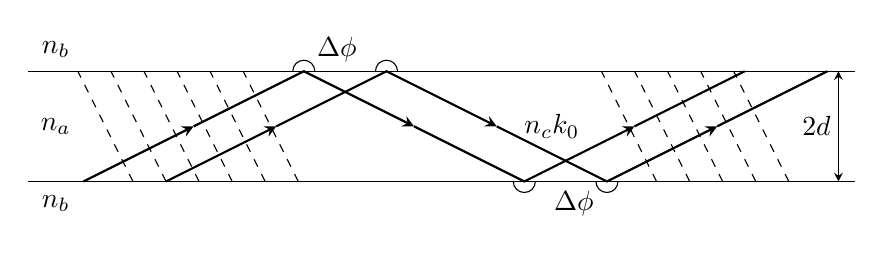
\begin{tikzpicture}[scale=0.7,>=stealth]
\draw (-9,0) -- (6,0) (-9,2) -- (6,2);
% \draw [->] (-9,1) -- (6,1);
\foreach \x in {0,1.5}{
  \draw [thick, ->] (-8+\x,0) -- (-6+\x,1);
  \draw [thick,->] (-6+\x,1) -- (-4+\x,2) -- (-2+\x,1);
  \draw [thick,->] (-2+\x,1) -- (0+\x,0) -- (2+\x,1);
  \draw [thick,-] (2+\x,1) -- (4+\x,2);
}
\foreach \x in {-1,0,1,2,3,4}
	\draw [dashed] (-6.5+0.6*\x,0) -- (-7.5+0.6*\x,2);
\foreach \x in {0,1,2,3,4}
	\draw [dashed] (2.4+0.6*\x,0) -- (1.4+0.6*\x,2);

% \draw [<->] (-9,1.5) --(-9,0.7) -- (-7.4,0.7);
% \draw [->] (-9,0.7) -- (-7.4,1.5);

% \node at (-8.6,1.4) {$\tiny{k_i}$};
% \node at (-8.2,0.4) {$\tiny{\beta}$};
\node at (0.5,1) {$n_c k_0$};

\draw [<->] (5.7,0) -- (5.7,2);
\node at (5.3,1) {$2d$};
\node at (-8.5,1) {$n_a$};
\node at (-8.5,2.4) {$n_b$};
\node at (-8.5,-0.4) {$n_b$};
\node at (-3.4,2.4) {$\Delta\phi$};
\node at (0.9,-0.4) {$\Delta\phi$};

\draw (-3.8,2) arc [start angle=0, end angle=180, radius=0.2];
\draw (-3.8+1.5,2) arc [start angle=0, end angle=180, radius=0.2];

\draw (-3.8+3.6,0) arc [start angle=180, end angle=360, radius=0.2];
\draw (-3.8+5.1,0) arc [start angle=180, end angle=360, radius=0.2];
\end{tikzpicture}
\caption{\textbf{Planar waveguide}. The upper and bottom layer are cladding and the middle is core layer. $\Delta \phi$ represents the Goos-H\"{a}nchen shift at the boundary.}
\label{fig:planar}
\end{figure}

Hence, we can study the eigenequantion by selecting only one set of boundary condition, as used in the \textit{the effective index method}. For example, in a planar waveguide shown in \autoref{fig:planar} ,$\dv*[2]{}{y}=0$\footnote{Since the planar waveguide is infinite at the $y$-direction , thus the solution is identical in arbitrary $xz$-plane, which means no gradient along $x$-axis.},
the TE mode features $E_x=0$ and consider only $y$-component, 
\begin{equation}
    \dv[2]{E_y}{x} + (k^2 n^2 - \beta^2)E_y =0
\end{equation}
and $E_y$ is continous at $x=\pm d/2$, where $d$ is the thickness of core layer.

For the region $|x|>d/2$, the light evanesces at $x$-direction at rate $\kappa$ and in contrast, in the region of core layer, the light performs like stationary wave, denoting with $k_x$. By substituting these conditions, phase continuity is achieved between two interface

\begin{equation}\label{eq:te-eq}
    2k_x d = m\pi + 2\arctan(\kappa/k_x)
\end{equation}
where $m$ is the index of stationary wave. The second term can be treated as the Goos-H\"{a}nchen phase shift. Overall, the waveguide modes characterize that the phase shall maintain itself with an $m\pi$ shift along with the shift at the boundaries.

In the case of TM modes, the eigen equation is 
\begin{equation}\label{eq:tm-eq}
    2k_x d = m\pi + 2\arctan(\delta\kappa/k_x)
\end{equation}
where $\delta=n_a/n_b$ is the index ratio and only differs from \autoref{eq:te-eq} with this parameter. conclusively, the less is $\delta$ parameter, the propagation constant of TE and TM modes are closer.

\subsection{Dispersion relation}
Based on \autoref{eq:te-eq} and \autoref{eq:tm-eq}, $k_x$ can be solved and then utilized to calculate propagation constant $\beta$, since $n_a^2k^2 = k_{\perp}^2 + \beta^2$. In the case of channel waveguides, the TE and TM solutions are both necessary. Therefore, propagation constants $\beta$ can be expressed as the product of free space wave vector $k$ and the \textit{ effective index} $n_{\mathrm{eff}}$
\begin{equation}\label{eq:disp_bk}
    \beta = n_{\mathrm{eff}}k = n_{\mathrm{eff}}(\lambda) \frac{2\pi}{\lambda} = n_{\mathrm{eff}}(\omega) \frac{\omega}{c}
\end{equation}
along with the differential form
\begin{equation}\label{eq:ng-def}
    \dv{\beta}{k} = n_{\mathrm{eff}} + k \dv{n_{\mathrm{eff}}}{k} = n_{\mathrm{eff}} - \lambda\dv{n_{\mathrm{eff}}}{\lambda} \equiv n_g
\end{equation}
which defines the group index $n_g$.

This formula linking $\beta - k$ or $\beta - \omega$ is named as dispersion relation, which gives the physics that light with different color propagates at different \textit{speed}. Furthermore, \autoref{eq:te-eq} and \autoref{eq:tm-eq} also indicate that the dispersion relation intrinsically depends on waveguide geometry.

\section{Ring resonators}

The ring resonators comprise of a bus waveguide and a ring waveguide, are usually demonstrated as optical filters or modulators at a wide range of platforms. The working principle of ring resonator can be derived completely \cite{Bogaerts2012} as an analogue to Fabry-P\'{e}rot etalon, based on the coupling mode theory. 

\begin{figure}
    \centering
	\includesvg{mrr_illus}
	\caption{\textbf{An all-pass type ring resonator.} The transmitted spectrum is filtered periodically by the ring waveguide, in the case satisfying resonance condition.}
    \label{fig:mrr-illus}
\end{figure}

In the model illustrated in \autoref{fig:mrr-illus}, the self-coupling coefficient $\tau$ and the cross-coupling coefficient $\kappa$ can be evaluated analytically or using numerical simulation. Assuming the coupling only occur at the very close area, $\tau,\kappa$ are the power splitting ratios of the coupler and satify $\tau^2 + \kappa^2 =1 $ if the coupling section is lossless. $a$ is the single-pass amplitude transmission, including both propagation loss in the ring and loss in the couplers.

\begin{figure}
    \centering
    \includesvg{mrr_cp}
    \caption{\textbf{The transmission spectrum of a ring resonator.} }
    \label{fig:mrr_spec}
\end{figure}

The transmission rate of a all-pass type ring cavity takes the form of
\begin{equation}\label{eq:trans_phi}
    T = \frac{I_\mathrm{pass}}{I_\mathrm{input}} = \frac{a^2 - 2a\tau \cos \phi + \tau^2}{1 - 2ar \cos \phi + a^2 \tau^2}
\end{equation}
where $\phi=\beta L$ is the phase shift in a single round trip. 

\subsection{Coupling condition}

By plotting the function in \autoref{fig:mrr_spec}, we can see, the extinction ratio of absorption peak is defined by the self-coupling coefficient $\tau$ and the single-pass amplitude transmission $a$ due to device geometric differences, like the gap between the bus waveguide and the ring cavity. Namely, $a$ and $\tau$ both determine the coupling condition, which can be categorized in three cases
\begin{itemize}
    \item \textbf{weak coupling} $a>\tau$. The loss inside the ring is larger than the power coupled from bus waveguides.
    \item \textbf{critical coupling} $a=\tau$. The loss and self-coupling are in balance. The optical power restored in the resonator achieve the minimum.
    \item \textbf{over coupling or strong coupling} $a<\tau$. The coupling is too strong for the light to dissipate in a single round trip.
\end{itemize}

Previous work \cite{Yusuke2017} proposed a method to evaluate the coupling condition above using the experimentally measured device transmission. Considering the loss in the coupler, bent segment of ring and higher mode perturbance, usually the critical coupling varies from modes and the cross section of waveguides \cite{Pfeiffer2017}.

\subsection{Spectrum characteristics}
Meanwhile, the minimum of transmission rate $T$ can be achieved periodically as $\phi=2 \mu \pi$, which defines the resonance of ring resonators. Therefore, the resonance condition is derived as
\begin{equation}
    \beta L =2 \mu \pi
\end{equation}
    
Specifically, the propagation constant $\beta$, shall be an integral times of a quasi wave vector $2\pi/L$. With this condition, the free spectrum range (FSR) of wavelength and frequency are obtained
\begin{align}
    \Delta \lambda_\mathrm{FSR} &\approx \frac{\lambda_\mathrm{res}^2}{n_g L} \label{eq:fsr-wl} \\
    \Delta \omega_\mathrm{FSR} &\approx \frac{n_g L}{2\pi c} \label{eq:fsr-w}
\end{align}

In both wavelength and frequency domain, FSR determines the spacing of neighbouring resonant peak. This is a significant factor when the ring resonators are designed.

Furthermore, from \autoref{eq:trans_phi}, the full width at half maximum (FWHM) of the resonance spectrum is derived as $\delta\lambda$
\begin{equation}\label{eq:fwhm_phi}
    \delta\phi = \frac{2(1- a \tau)}{\sqrt{\tau a}}
    % \lambda_{\mathrm{res}}^2
\end{equation}
\begin{figure}
    \centering
    \includesvg{mrr_fsr_illus}
    \caption{Caption}
    \label{fig:my_label}
\end{figure}

Likely, since the phase $\phi$ is related with the wave vector $k$ in \autoref{eq:ng-def}. Substituting $\delta \phi = L n_g \delta k$, the half width of wavelength is
\begin{equation}
    \delta \lambda = \dv{\lambda}{k}\delta k = \frac{\lambda_\mathrm{res}^2}{2\pi L n_g} \frac{2(1- a \tau)}{\sqrt{\tau a}} \label{eq:fwhm_wl}
\end{equation}
the same, at the frequency domain
\begin{equation}
    \delta \omega = \dv{\omega}{k}\delta k = \frac{c}{ L n_g} \frac{2(1- a \tau)}{\sqrt{\tau a}} \label{eq:fwhm_w}
\end{equation}

Note in \autoref{eq:fsr-wl} \autoref{eq:fsr-w} \autoref{eq:fwhm_wl} and \autoref{eq:fwhm_w}, the group index $n_g$ is explicit instead of the effective index $n_\mathrm{eff}$ because both free spectrum range and full width depend on the differential form, \autoref{eq:ng-def}.

And the finesse $F$ of the resonator is defined 
\begin{equation}
    F \equiv \frac{2\pi}{\delta\phi} = \frac{\pi\sqrt{\tau a}}{2(1- a \tau)}
\end{equation}

Finally, we define the quality factor, a measure of the sharpness of the resonance relative to its central frequency.

\begin{equation}\label{eq:q-def}
    Q = \frac{\lambda_\mathrm{res}}{\delta \lambda} =  \frac{\pi L n_g \sqrt{\tau a}} {\lambda_\mathrm{res} (1- a \tau)}
\end{equation}

Usually, the \textit{Q}-factor can be decomposed into two parts by formula $Q^{-1}=Q_{i}^{-1} + Q_{l}^{-1}$. And $Q_{i}, Q_{l}$ are intrinsic \textit{Q}-factor and loaded \textit{Q}-factor, referring to the loss inside the ring waveguide and at the coupler, respectively. The physical meaning of the finesse and \textit{Q}-factor relates to the number of round-trips before being lost to internal loss and the bus waveguides when the power is depleted to $1/e$ of its initial value.

\section{Thrid-order nonlinear optics}

Although the nonlinear effect is ignored during the derivation of waveguide modes in \autoref{sec:guide}, 
for numerous materials, the nonlinear response of electric field is significant even at mW level, which is easy to occur with assistance of modern lasers. The origin of nonlinear optic phenomena is similar to the movement of the object in a potential field, such as the ball-spring model. 

In the nonlinear material, the atoms or molecules are driven by the external electric field, due to the around chemical bonds or molecular orientation, the displacement of atoms or molecules perform nonlinear dependence on the strength of field. In real-world materials, interaction coming arising from various frequency leads to the addition or subtraction of these frequency components. This explains the frequency conversion nature in nonlinear optics.

% these phenomena are widely used in quantum optics, such as spontaneous parametric down conversion. And
It is worth mentioning that not only in the bulk crystals, but also in the sub-micron scale \cite{Leuthold2010}, the nonlinear response is still efficient, even over a single-layer two-dimensional material.

% In this section, we prefer to introduce both second-order and third-order optical nonlinearity. 
Here, a brief theoretical derivation is elucidated and in the following part, degenerate four wave mixing is emphasized. In an isotropic nonlinear medium, assuming only instantaneous dielectric response, the relation between the polarization and the electric field is expressed by a power series in the electric field
\begin{equation}\label{eq:nlp}
    \vb{P} = \varepsilon_0 \large (\chi^{(1)}\vb{E} + \chi^{(2)}\vb{E}^2 + \chi^{(3)}\vb{E}^3)
    = \varepsilon_0 \chi^{(1)}\vb{E} + \vb{P}_\mathrm{NL}
\end{equation}

Note in \autoref{eq:nlp}, the nonlinear susceptibilities $\chi^{(2)}$ and $\chi^{(3)}$ are second-rank and third-rank tensors, corresponding to the tensor product with $\vb{E}^2$ and $\vb{E}^3$. The higher order response is neglected and sequentially, only $\chi^{(2)}$ processes and $\chi^{(3)}$ processes are to be introduced.

\bigskip
\noindent\textbf{$\chi^{(2)}$ processes} 

In centrosymmetric crystals such as silicon, the second-order susceptibility term is absent. However, in other materials like lithium niobate (\ce{LiNbO3}) and aluminium nitride (AlN), the second-order nonlinearity are essential to realize electro-optic modulation and second harmonic generation.

\bigskip
\noindent\textbf{$\chi^{(3)}$ processes} 

Silicon and silicon nitride are both cubic crystal. Due to the third-order dependence, another factor equivalent to the optical intensity is involved, the $\chi^{(3)}$ process is also named as intensity-dependent effect or Kerr effect.

Consider three frequency components of $\vb{E}^3$, using the complex expression of electric field
\begin{equation}
    \vb{E}(\vb{r}, t) = \sum_{k=1}^3 \vb{E}_{\omega_k}(\vb{r}, t) =  \frac{1}{2} \sum_{k=1}^3 \qty ( \vb{E}_{\omega_k}(\vb{r})e^{i\omega_k t} + c.c.)
\end{equation}

Substituting into third-order term in \autoref{eq:nlp} and arranging with the same propagation direction, the third-order polarization is 

\begin{align}
  \vb{P}^{(3)} 
  & = \frac{3}{4} \varepsilon_0 \chi^{(3)} \left[| \vb{E}_{\omega_1} |^2 \vb{E}_{\omega_1} + \cdots\right] & \mathrm{SPM} \\
  & + \frac{6}{4} \varepsilon_0 \chi^{(3)} \left[(| \vb{E}_{\omega_2} |^2 + |\vb{E}_{\omega_3} |^2) \vb{E}_{\omega_1} + \cdots \right] & \mathrm{XPM} \\
  & + \frac{1}{4} \varepsilon_0 \chi^{(3)} \left[(\vb{E}_{\omega_1}^3 e^{i \omega_1 t} + c.c.) + \cdots\right] & \mathrm{THG} \\
%   \tag{\stepcounter{equation}\theequation}
  & + \frac{3}{4} \varepsilon_0 \chi^{(3)} \left[ \frac{1}{2} (\vb{E}_{\omega_1}^2 \vb{E}_{\omega_2} e^{i (2 \omega_1 + \omega_2) t} + c.c.) + \cdots \right] & \mathrm{FWM} \label{eq:fwm1} \\ 
  & + \frac{3}{4} \varepsilon_0 \chi^{(3)} \left[ \frac{1}{2} (\vb{E}_{\omega_1}^2 \vb{E}^{\ast}_{\omega_2} e^{i (2 \omega_1 - \omega_2) t} + c.c.) + \cdots \right] & \mathrm{FWM} \label{eq:fwm2} \\ 
  & + \frac{6}{4} \varepsilon_0 \chi^{(3)} \left[ \frac{1}{2} (\vb{E}_{\omega_1} \vb{E}_{\omega_2} \vb{E}_{\omega_3} e^{i (\omega_1 + \omega_2 + \omega_3) t} + c.c.) + \cdots \right] & \mathrm{FWM}  \label{eq:fwm3} \\
  & + \frac{6}{4} \varepsilon_0 \chi^{(3)} \left[ \frac{1}{2} (\vb{E}_{\omega_1} \vb{E}_{\omega_2} \vb{E}^{\ast}_{\omega_3} e^{i (\omega_1 + \omega_2 - \omega_3) t} + c.c.) + \cdots \right] & \mathrm{FWM} \label{eq:fwm4}
\end{align}

In above equations, $\cdots$ stands for all possible permutation terms contributed by frequencies $\omega_1, \omega_2, \omega_3$. The abbreviation on the right side represent for 

\bigskip
\noindent\textbf{SPM, self-phase modulation}

SPM adds an intensity-dependent term except the linear polarization, leading to a broadening of the pulse spectrum.

Note the $\chi^{(3)}$ is complex, thus the imaginary part may contribute to another intensity-dependent absorption mechanics, which is usually depicted in the \textit{two-photon absorption} (TPA). The free carriers excited by TPA in further change the temporally both the absorption coefficient and the refractive index of material.
\begin{equation}\label{eq:spm-index}
    n = n_0 + n_2 I + i \frac{\lambda}{4\pi}(\alpha_0 + \alpha_2 I)
\end{equation}
where the $I$ is the intensity, $n_2$ is the Kerr coefficient and $\alpha_0, \alpha_2$ are related with TPA-induced free carrier absorption (FCA) and free carrier index (FCI) change, both interrelated with third-order susceptibility
\begin{align}
    n_2     &= \frac{1}{cn_0^2\varepsilon_0} \frac{3}{4} \Re{\chi^{(3)}} \\
    \alpha_2&= \frac{-\omega}{c^2n_0^2\varepsilon_0} \frac{3}{2} \Im{\chi^{(3)}}
\end{align}
A figure of merit (FOM) is often used to compare the magnitude of Kerr coefficient $n_2$ with the strength of the TPA coefficient $\alpha_2$
\begin{equation}
    \mathrm{FOM} = \frac{1}{\lambda} \frac{n_2}{\alpha_2}
\end{equation}

\bigskip
\noindent\textbf{XPM, cross-phase modulation} 

XPM can be seen the first signal index influenced by a second signal. And the coeffiecient of XPM is twice as strong as the SPM coefficient.

\bigskip
\noindent\textbf{THG, third-harmonic generation} 

Like SHG, THG generated a new frequency with is one-third of input frequency. 

\bigskip
\noindent\textbf{FWM, four wave mixing} 

% \item DFWM, degenerate four wave mixing
% Another factor to mention is that the coefficient in each $\chi^{(3)}$ process arises from the combination of three frequency components. For instance, on the numerator \autoref{eq:def-dfwm} has the factor 3 but \autoref{eq:def-ndfwm} has the factor 6. 
In FWM process, more than three frequencies are involved. Nevertheless, \autoref{eq:fwm1} and \autoref{eq:fwm2} contain two identical wave, sometime calles as degenerate four wave mixing (DFWM). And \autoref{eq:fwm3} and \autoref{eq:fwm4} is a truly four wave process. Similar to the relation between SPM and XPM, the non-degenerate FWM is naturally twice stronger.

Traditionally, following the terminology in laser field, in DFWM, the $\omega_1$ square term \autoref{eq:fwm2} is labeled as pump frequency, and another two frequencies are referred to signal and idler frequency.

Besides, the imaginary part of third-order susceptibility incorporate other four-wave absorption mechanics, such as \textit{stimulated Brillouin scatter} (SBS) and \textit{stimulated Raman scattering} (SRS), which originate from acoustic waves in crystals and vibrating molecules.

Finally, it worth mentioning that in all THG and FWM processes, different from SPM and XPM processes, phase matching condition is required due to the complex exponential factors. In this case, the phase mismatch can change the polarization rapidly and leads to periodical variation in these parametric processes.

\section{Nonlinear integrated devices}

From the above section, in the nonlinear optical waveguide or just silica fiber,
phase matching condition of degenerate four wave mixing involves not only the SPM of pump light and XPM of signal and idler light, but also the phase mismatch in FWM propagation factor\cite{Agrawal2013a}. 

However, in our research objective, the resonator limits the mode linewidth (pm), which is much narrower than SPM frequency broadening. Based on this fact, we neglect the pump light broadening in the cavity. And the phase matching condition is dealt with in \autoref{chap:pmc-sfwm}.


\chapter{Phase match condition for spontaneous four wave mixing in a ring cavity }
\section{Chromatic dispersion}

\section{Broadband phase matching condition}
\section{Dispersion compensation and engineering using slot structure}
\section{Effects of mode crossing}
\section{Four wave mixing}


Assume in a ring resonator, to satisfy both energy conservation and momentum
conservation,
\begin{eqnarray*}
  \beta_i + \beta_s & = & 2 \beta_p\\
  \omega_i + \omega_s & = & 2 \omega_p
\end{eqnarray*}
meanwhile, $\beta = m \frac{2 \pi}{L}$, and $L$ is the length of the
resonator. Thus,

{\tmname{\begin{equation}
  m_i + m_s = 2 m_p
\end{equation}}}

Hence, \tmtextit{the momenmtum conservation agrees with mode numder
equidistant.} Thus, we choose the frequency domain to estimate the phase
mismatch. Expand the frequency into Taylor seires at $\omega_0$ to the
propagation constant $\beta$,
\begin{eqnarray}
  \omega_{\mu} & = & \omega_0 + \frac{\mathd \omega}{\mathd \beta}
  (\beta_{\mu} - \beta_0) + \frac{1}{2}  \frac{\mathd^2 \omega}{\mathd
  \beta^2} (\beta_{\mu} - \beta_0)^2 + \cdots \\
  & = & \omega_0 + \frac{\mathd \omega}{\mathd \beta} \frac{2 \pi}{L} \mu +
  \frac{\mathd^2 \omega}{\mathd \beta^2} \left( \frac{2 \pi}{L} \mu \right)^2
  + \cdots \nonumber\\
  & = & \omega_0 + D_1 \mu + D_2 \mu^2 + D_3 \mu^3 + \cdots \nonumber
\end{eqnarray}
where $D_1 / 2 \pi = 1 / v_g L$ is the \tmtextit{free spectrum range}, and
\begin{eqnarray*}
  \tmop{as} & = & a
\end{eqnarray*}

\bibliography{library}
\bibliographystyle{abbrv}

\clearpage % ensure all floats are processed
% \processdelayedfloats
\clearpage

\appendix

\chapter{Supple}
\end{document}
